\subsubsection{Неоднородное уравнение.}
		\[
			\derp{u}{t}{2} = a^2 \derp{u}{x}{2} + h(x, t)
		\]
		\[
			t = 0 \quad u(x, 0) = f(x) \quad \derp{u}{t}{} (x, 0) = g(x)
		\]
		\begin{figure}[h!] 
			\centering 
			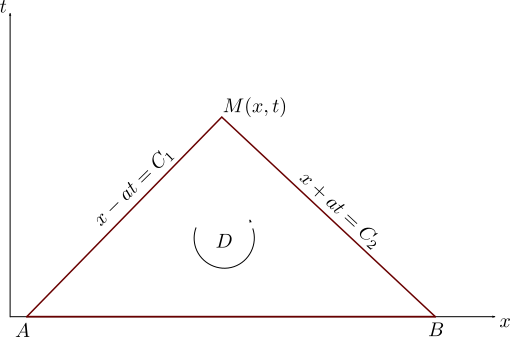
\includegraphics[width=0.6\textwidth]{figStringKoshi.pdf}
			\caption{Характеристический треугольник}
		\end{figure}\\
		Проинтегрируем обе части уравнения по области, заключённой внутри характеристического треугольника и разделим обе части на $2 a$.
		\[
			\frac{1}{2a} \iint\limits_D \derp{u}{t}{2} dx dt = \frac{a}{2} \iint\limits_D \derp{u}{x}{2} dx dt + \frac{1}{2 a} \iint\limits_D h(x, t) dx dt
		\]
		По формуле Грина 
		\[
			\iint\limits_D \derp{u}{t}{2} dxdt = - \oint\limits_{\partial D} \derp{u}{x}{} dt \qquad \iint\limits_D \derp{u}{x}{2} dx dt = \oint\limits_{\partial D} \derp{u}{x}{} dt
		\]
		\[
			- \oint_{\partial D} \derp{u}{t}{} = - \left[ \int\limits_A^B \derp{u}{t}{} dx + \int\limits_B^M \derp{u}{t}{} dx + \int\limits_M^A \derp{u}{t}{} dx \right] = 
		\]
		\[ 
			= - \int\limits_A^B \derp{u}{t}{} dx + a \int\limits_B^M \derp{u}{t}{} dt - a \int\limits_M^A \derp{u}{t}{} dt = 
		\]
		\[ 
			= - \int\limits_A^B \derp{u}{t}{} dx + 2 a u(M) - a u(A) - a u(B)
		\]
		\begin{multline*}
			\oint_{\partial D} \derp{u}{x}{} dt = \cancelto{0}{\int\limits_A^B \derp{u}{x}{} dt} + \int\limits_B^M \derp{u}{x}{} dt + \int\limits_M^A \derp{u}{x}{} dt = - \frac{1}{a} \int\limits_B^M \derp{u}{x}{} dx + \frac{1}{a} \int\limits_M^A \derp{u}{x}{} dx = \\ 
			=- \frac{2}{a} u(M) + \frac{(u(A) +u(B))}{a} = \frac{1}{2 a} \int\limits_A^B \derp{u}{t}{} dx + u(m) - \frac{u(B) +u(A)}{2} =\\=
			 - u(M) + \frac{u(B)+u(A)}{2}  + \frac{1}{2a} \iint\limits_D h(x, t) dx dt
		\end{multline*}
		\[
			2 u(M) = \frac{1}{2a} \int\limits_A^B \derp{u}{t}{} dx + u(A) +u(B) + \frac{1}{2a} \iint\limits_D h(x, t) dx dt
		\]
		\[
			x_m - at_m = C_1 = x - at \Rightarrow x_A = x_m - at_m
		\]
		\[
			x_m + at_m = C_2 = x + at \Rightarrow x_B = x_m - at_m
		\]
		\[
			u(M) = \frac{u(x_m +at_m) + u(x_m - a t_m)}{2} + \frac{1}{2a} \int\limits_{x_m - at_m}^{x_m + a t_m} g(\xi) d \xi + \frac{1}{2a} \iint\limits_D h(x, t) dx dt
		\]


\subsubsection{Задача распространения волн в полубесконечной струне.}
		Пусть $f(x)$ и $g(x)$ - нечётные
		\[
			u(0, t) = \frac{f(at) +f(-at)}{2} + \frac{1}{2a} \int\limits_{-at}^{at} g(\xi) d\xi = 0
		\]
		Можно продолжить $f(x)$ нечётным образом:
		\[
			f_1(x) = sgn(x) \cdot f(\abs{x})
		\]
		Аналогично для $g_1(x) = sgn (x) \cdot g(\abs{x})$
		\begin{enumerate}
			\item $x - at > 0$ - решение записывается в обычном виде\\
			\item $x - at < 0: x > 0, t > \frac{x}{a}$
		\end{enumerate}
		\begin{multline*}
			u(x, t) = \frac{f(x + at) + f(x - at)}{2} + \frac{1}{2a} \int\limits_0^{x +at} g_1(\xi) d \xi + \frac{1}{2 a} \int\limits_{x - at}^0 g_1 (\xi ) d\xi =\\= [-z = \xi \quad -dz = d\xi ] 
			= \frac{f(x + at) + f(x - at)}{2} +  \frac{1}{2a} \int\limits_0^{x +at} g_1(\xi) d \xi + \frac{1}{2 a} \int\limits_0^{at -x} g (z ) dz
		\end{multline*}
		Рассмотрим начальные условия: 
		\[
			x = 0; \quad \derp{u}{t}{} = 0
		\]
		Вместо $x = 0; \quad u(0, t)$\\
		$g(x), f(x)$ - чётные\\
		\[
			\derp{u}{t}{} = \frac{a f' - a f'}{2}
		\]

        \[
			u(x,t)= X(x) Y(t)
		\]
		\[
			\begin{cases}
				\frac{Y''}{a^2 Y} = \frac{X''}{X} = - k^2\\ 
				X(0) = 0, X(l) = 0
			\end{cases}
		\]
		\[
			X_k = C_{1k}^* \cos kx + C_{2k}^* \sin k x
		\]
		\[
			X(0) = 0 \Rightarrow C_1^*
		\]
		\[
			X(l) = 0 \Rightarrow C_{2k}^*\sin k l = 0
		\]
		\[
			k l=\pi n \Rightarrow k_n=\pi\frac{n}{l}
		\]
		$k_n$ -- cобственные числа.
	    \[
			n \in N \Rightarrow X_n= C_{2n}^* \sin \frac{\pi n}{l} x
		\]
		\[
			Y_n = A_k\cos \frac{a\pi k}{l} t + B_k \sin\frac{a\pi k}{l} t,
		\] 
		\begin{align*}
			&A_n C_{2n}^* =C_{1n}\\
			&B_n C_{2n}^* = C_{2n}
		\end{align*}
		
		\[
			u_n (x, t) = \left(C_{1n} \cos \frac{a \pi n}{l} t + C_{2n} \sin \frac{a \pi n}{l} t \right) \sin\frac{\pi n}{l} x
		\]
		\[
			u(x, t) = \sum\limits_{n = 1}^{\infty} u_n (x, t) = \sum\limits_{n = 1}^{\infty} \left(C_{1n} \cos \frac{a \pi n}{l} t + C_{2n} \sin \frac{a \pi n}{l} t \right) \sin\frac{\pi n}{l} x
		\]
		Рассмотрим начальное условие $u(x,0) = f(x)$\\
		\[
			f(x) = \sum\limits_{n = 1}^{\infty} C_{1n} \sin \frac{\pi n}{l} x
		\]
		\[
			\int\limits_0^1 f(x) \sin \frac{\pi n}{l} x dx = C_{1n} \frac{l}{2} \Rightarrow C_{1n} = \frac{2}{l} \int\limits_0^l f(x) \sin \frac{n \pi}{l} x dx
		\]
		Коэффициенты $C_{2k}$ находят из 2-го условия $\derp{u}{t}{} |_{t = 0} = g(x)$\\
		\[
			g(x) = \sum\limits_{n = 1}^{\infty}\left(C_{2n}\cos \frac{a \pi n}{l} t - C_{1n} \sin \frac{a \pi n}{l} \right) \frac{a \pi n}{l} \sin \frac{\pi n}{l} x |_{t = 0}
		\]
		\[
			g(x) = \sum\limits_{n = 1}^{\infty} C_{2n} \frac{a \pi n}{l} \sin \frac{\pi n}{l} x
		\]
		\[
			\int\limits_0^l g(x) \sin \frac{\pi k}{l} x dx = \frac{a \pi k}{l} C_{2k} \cdot \frac{l}{2}
		\]
		\[
			C_{2k} = \frac{2}{a \pi k} \int\limits_0^l g(x \sin \frac{\pi k}{l} x dx)
		\]
		Проверить, совпадает ли с решением Д'Аламбера.

		\[	
			u(x, t) = \frac{f(x + at) + f(x - at)}{2} + \frac{1}{2a} \int\limits_{x - at}^{x + at} g(\xi) d \xi
		\]
		\[
			f(x) = \sum\limits_{n = 1}^{\infty} C_{1n} \sin \frac{\pi n}{l} x \quad g(x) = \sum\limits_{n = 1}^{\infty} C_{2n} \frac{a \pi n}{l} \sin \frac{\pi n}{l} x\
		\]
		\begin{multline*}
			u(x,t) = \frac{1}{2} \left[ \sum\limits_{n = 1}^{\infty} C_{1n} \sin \frac{\pi n}{l} (x - at) + \sum\limits_{n = 1}^{\infty} C_{1n} \sin \frac{\pi n}{l} (x + at)\right] + \frac{1}{2a} \int\limits_{x - at}^{x + at} \sum\limits_{n = 1}^{\infty} C_{2n} \frac{a \pi n}{l} \sin \frac{\pi n}{l} \xi d \xi =\\
			= \sum\limits_{n = 1}^{\infty} C_{1n} \sin \frac{\pi n}{l} x \cos at \frac{\pi n}{l} +\frac{\pi}{a 2 l} \sum\limits_{n = 1}^{\infty} \int\limits_{x - at}^{x + at} C_{2n} n \sin\frac{\pi n}{l}\xi d \xi =\\
			= \sum\limits_{n = 1}^{\infty}C_{1n} \sin \frac{\pi n}{l} x \cos \frac{a \pi n}{l} t - \frac{a \pi}{a 2 l} \sum\limits_{n = 1}^{\infty} C_{2n} \frac{l}{\pi} \cos \frac{\pi n}{l} |_{x - at}^{x + at} =\\
			= \sum\limits_{n = 1}^{\infty} ( C_{1n}\sin \frac{\pi n}{l} x \cos\frac{a \pi n}{l} t + C_{2n} \sin \frac{\pi n}{l} x \cdot \sin \frac{\pi n a}{l} t) =\\
			= \sum\limits_{n = 1}^{\infty} \left(C_{1n} \cos \frac{\pi n a}{l} t C_{2n} \sin \frac{\pi n a}{l} t \right) \sin \frac{\pi n}{x}
		\end{multline*}
		Докажем сходимость рядов и единственность решения.
